\begin{abstract}
We estimate cosmic-muon coincidence rates in the ESA test stand with the
ECAL centred on the tracker axis and the remaining detectors at their original
heights. A golden cosmic event crosses all 26 active layers. Its estimated rate
is \goldNo{} per hour without an overhead slab and \goldRoof{} per hour beneath
3 ft of concrete. Requiring only the ten HCAL layers gives \hcalNo{} and
\hcalRoof{} per hour, respectively. We compare HCAL trigger definitions,
relax the tracker and other detector requirements, and tabulate every combination
of the three HCAL stations, the TS, LYSO and ECAL requirements, and tracker
multiplicity. The calculation uses the registered detector geometry, a sea-level
muon spectrum and continuous-range estimates along each trajectory. These are
muon-crossing rates before detector response; measured trigger
rates will also depend on thresholds, efficiency, noise and live time.
\end{abstract}

\section*{Overview}
The stand combines a compact trigger-scintillator (TS), silicon-tracker and
LYSO assembly with an ECAL module and three much larger HCAL stations.
The HCAL spans metres, while the TS bars are only 30 mm wide in $X$.
A muon crossing all the central devices must therefore pass through a narrow
common aperture.
Figures~\ref{fig:overview} and~\ref{fig:summary} show how this aperture controls the rate. This difference sets the scale of the commissioning samples: an HCAL
coincidence collects many muons, while a golden event connects every detector
through a single track.

For choosing a trigger, Table~\ref{tab:hcal} gives the rates for different HCAL
coincidences. For planning measurements with the central devices,
Table~\ref{tab:principal} gives the rate retained by each added requirement.
Both tables compare no overhead slab with the assumed 3 ft concrete slab and quote
rates before detection losses. The full set of combinations is collected in
Appendix~\ref{app:all}; the geometry, flux and stopping assumptions are described
in Sections~\ref{sec:layout} and~\ref{sec:method}.

% Keep the overview and the combined acceptance/rate figure consecutive.
\clearpage
\begin{figure}[p]
\centering
\begin{minipage}[t]{0.48\linewidth}
\centering\small\textbf{Aligned geometry used for the rates}\par\medskip
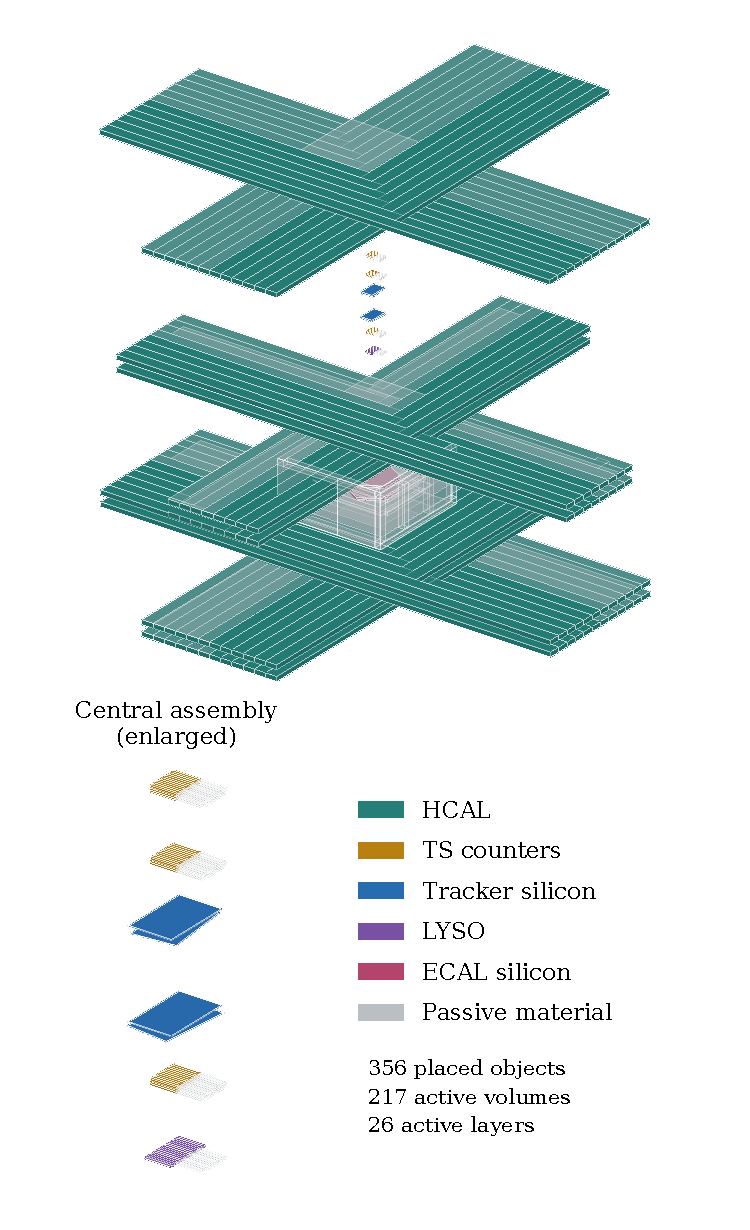
\includegraphics[width=\linewidth]{combinations_20260919/figures/full_installed_geometry.pdf}
\end{minipage}\hfill
\begin{minipage}[t]{0.49\linewidth}
\centering\small\textbf{Earlier offset layout: accepted rays}\par\medskip
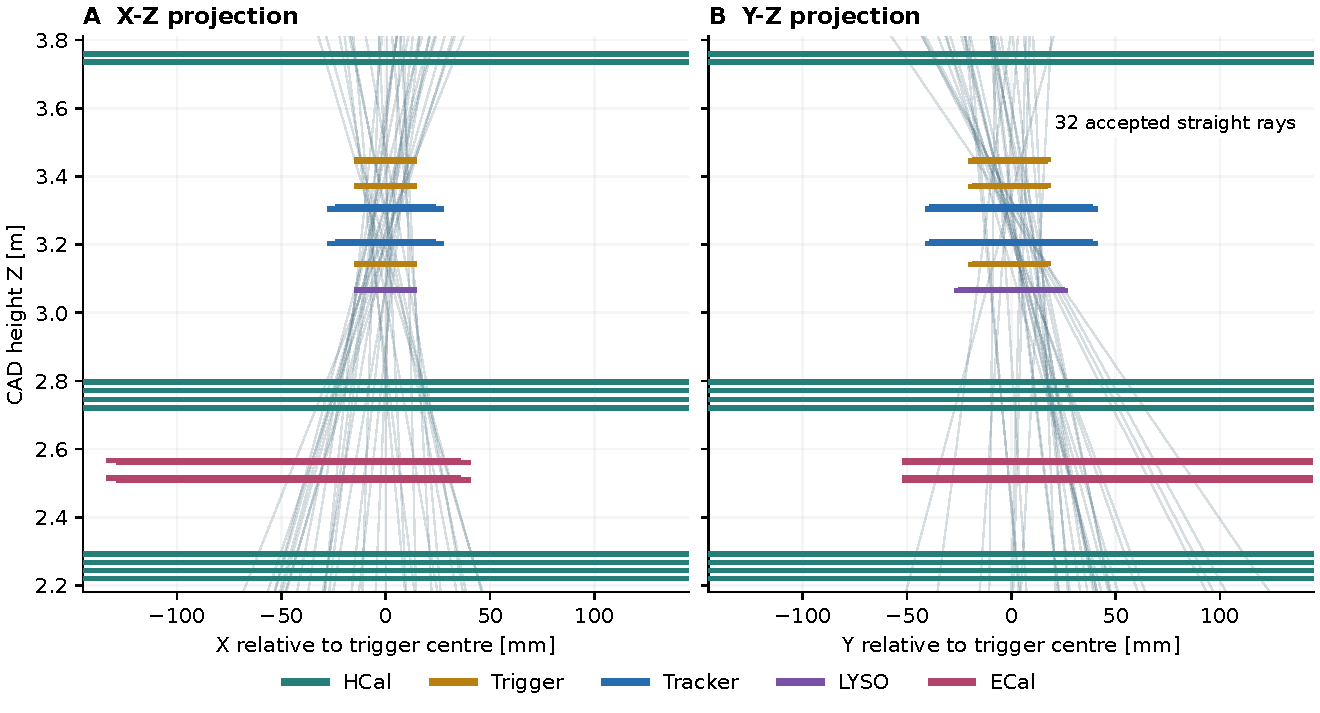
\includegraphics[height=2.88in,trim=0 26 300 0,clip]{geometry_acceptance.pdf}\par\medskip
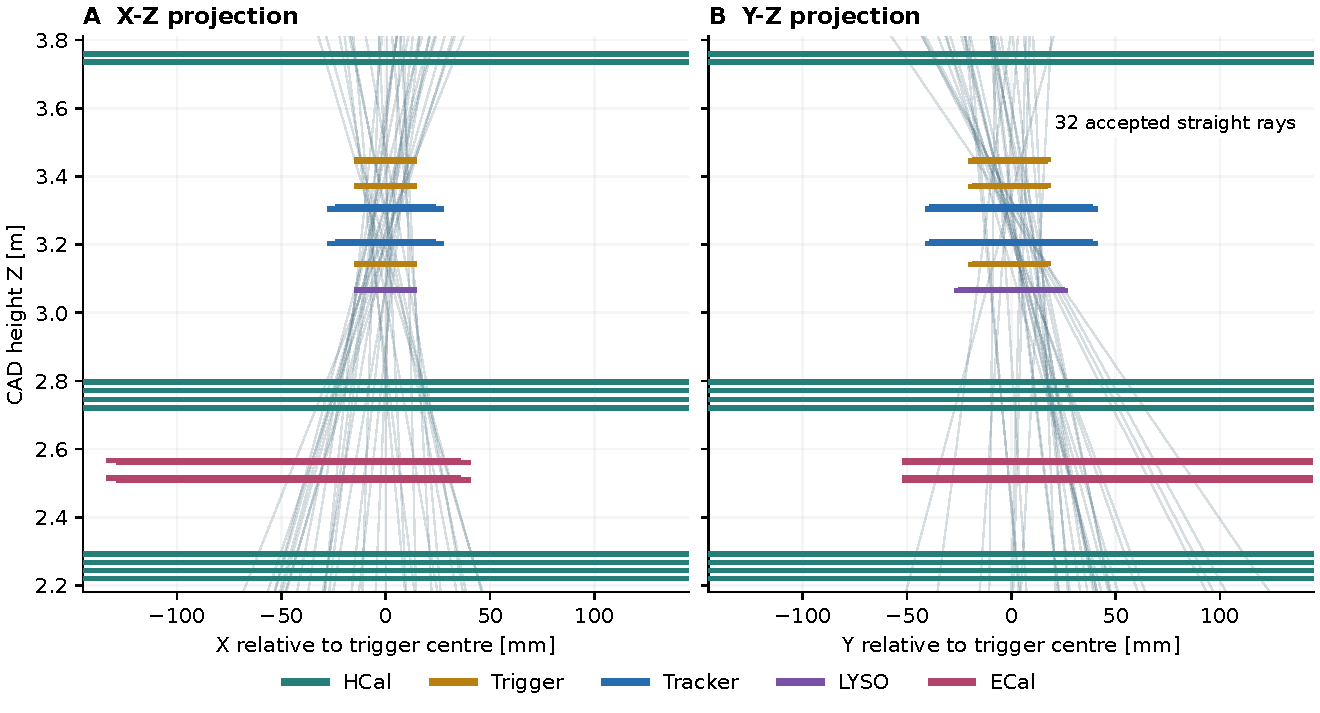
\includegraphics[height=2.88in,trim=336 26 0 0,clip]{geometry_acceptance.pdf}
\end{minipage}
\caption{\textbf{Installed geometry and the accepted-ray aperture.}
Left: the complete aligned detector model, with passive material shown
translucently and a separate enlargement of the central assembly below.
CAD stand supports are outside the material model. Right: the previous rate
report's 32 accepted straight rays, with its original vector projections
stacked for readability. These rays use the earlier \emph{offset} ECAL;
all main-table rates use the aligned layout. Colours identify the same
subsystems in both panels. The rays include no scattering or detector response.}
\label{fig:overview}
\end{figure}
\clearpage
\begin{figure}[p]
\centering
{\small\textbf{(a) Active-layer envelopes in the aligned layout}}\par\smallskip
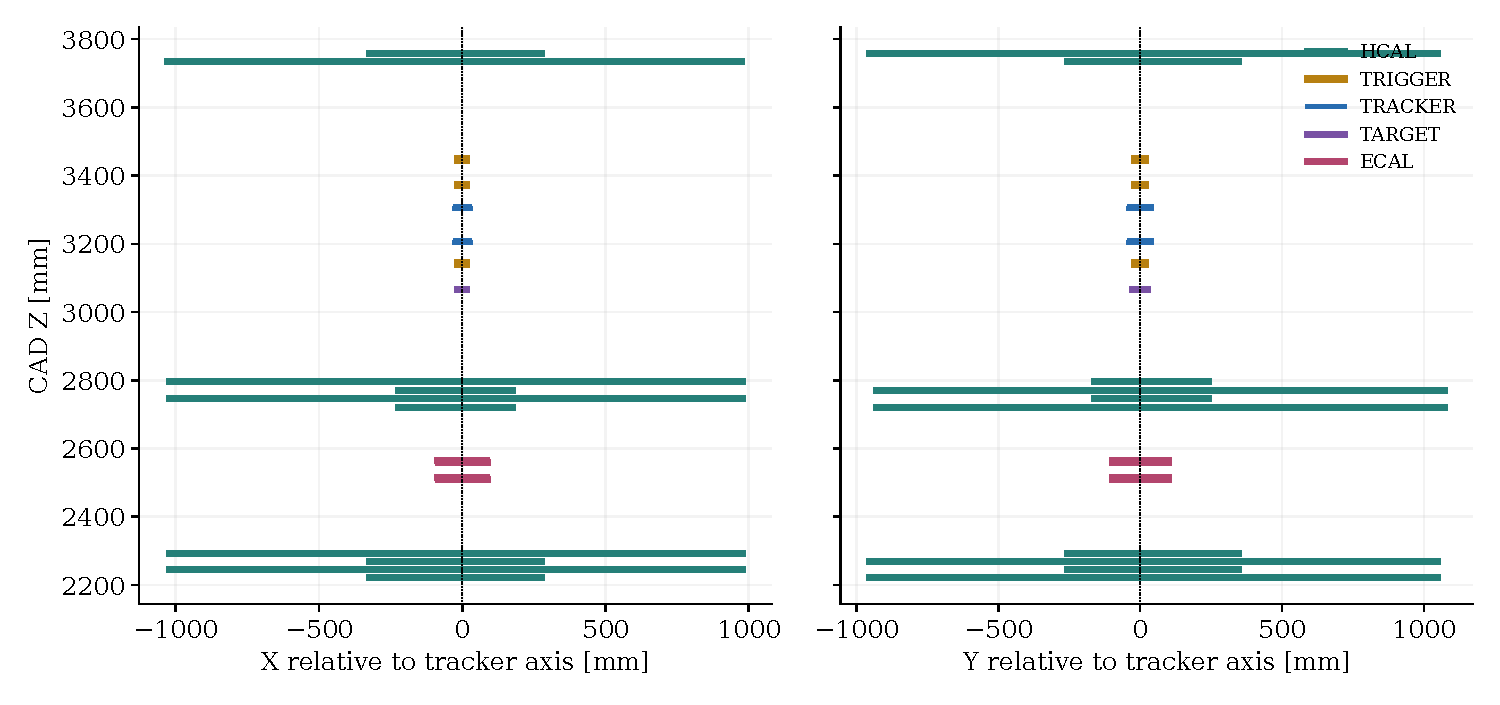
\includegraphics[width=0.98\linewidth]{combinations_20260919/figures/aligned_geometry.pdf}\par\medskip
{\small\textbf{(b) Rates retained by representative detector requirements}}\par\smallskip
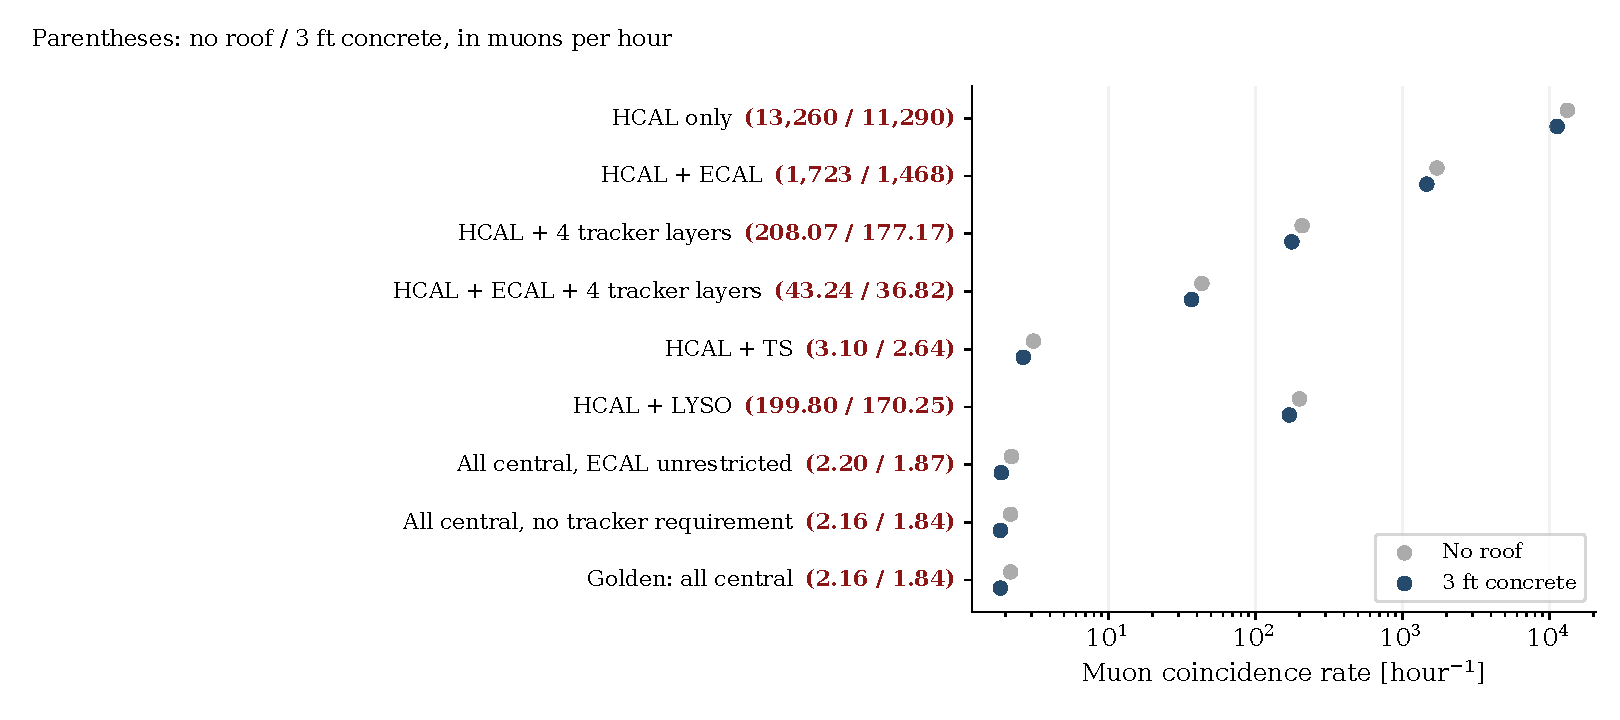
\includegraphics[width=0.98\linewidth]{combinations_20260919/figures/rate_hierarchy.pdf}
\caption{\textbf{From detector aperture to coincidence rate.}
(a) The active-layer envelopes, with transverse coordinates measured from
the tracker axis and heights in CAD $Z$. Line thicknesses are enlarged for
visibility; the calculation retains the segmented solids.
(b) Inclusive selections requiring all ten HCAL layers, on a logarithmic rate
axis. ``All central'' requires all TS, LYSO, ECAL and tracker layers.
``ECAL unrestricted'' keeps ECAL installed but imposes no ECAL hit requirement:
events may hit or miss it, while all other listed hit requirements still apply.
``No tracker requirement'' similarly leaves tracker hits unrestricted. The same aligned
geometry and sea-level spectrum are used for both roof assumptions. Bold red
values beside each selection give the rate per hour (no roof / 3 ft concrete).}
\label{fig:summary}
\label{fig:geometry}
\label{fig:hierarchy}
\end{figure}
\clearpage


\section{Reference layout and event definitions}
\label{sec:layout}
The reference configuration moves the entire ECAL by
$\Delta X=+46.5596$ mm and $\Delta Y=-46.0763$ mm in the CAD coordinate system.
Its combined active-silicon envelope is then centred on the tracker/TS/LYSO
axis at $(X,Y)=(5027.51999,-155.75023)$ mm. The four ECAL silicon layers
retain their internal offsets. No detector moves vertically, and all three
HCAL stations remain in place. This is the previously studied ``centred only''
layout; the raised assembly is retained as a historical comparison in
Appendix~\ref{app:previous}.

\begin{table}[htbp]
\centering\small
\caption{Active detector inventory. Heights are CAD $Z$; within each range, layers are ordered from top to bottom.}\label{tab:inventory}
\begin{tabular}{lrrl}
\toprule
Requirement & Layers & Active volumes & Height range (mm)\\
\midrule
$H_T$: top HCAL & 2 & 24 & 3758.711--3735.339\\
$S$: TS counters & 6 & 72 & 3449.388--3140.588\\
$T_1,T_2,T_3,T_4$: tracker & 4 & 4 & 3309.888--3203.888\\
$Y$: LYSO & 2 & 33 & 3066.788--3065.988\\
$H_M$: HCAL above ECAL & 4 & 32 & 2796.346--2720.146\\
$E$: ECAL silicon & 4 & 4 & 2566.032--2508.962\\
$H_B$: HCAL below ECAL & 4 & 48 & 2291.504--2220.931\\
\midrule
Golden event & 26 & 217 & All requirements\\
\bottomrule
\end{tabular}
\end{table}


We call an event \emph{golden} when one downward-going muon crosses an active
volume in every layer in Table~\ref{tab:inventory}. In a segmented layer,
crossing any one bar is sufficient. A hit requires a positive path length in
the active volume; it does not require passage through the layer midplane.
The inactive silicon borders do not count as tracker hits.

Throughout this note, ``everything minus ECAL'' means that ECAL hits are
unrestricted. The ECAL and its passive material remain installed. Likewise,
``minus one tracking layer'' means at least three of the four tracker layers,
with any one layer allowed to lack a hit. It includes four-layer events.
These inclusive samples overlap and must not be added. The separate
\texttt{exclusive\_tracker\_counts.csv} table gives exact tracker multiplicities;
physically removing equipment is a different geometry study.

The three HCAL stations are denoted $H_T$ (top, two layers), $H_M$ (above ECAL,
four layers) and $H_B$ (below ECAL, four layers). Unless explicitly stated
otherwise, requiring a station means requiring \emph{all} its active layers.
The TS requirement $S$ means all six trigger-scintillator layers; $Y$ means both
LYSO layers; $E$ means all four ECAL silicon layers. A tracker multiplicity
$T_{\ge k}$ accepts any set of at least $k$ of the four active tracker layers.



\section{HCAL trigger rates}
\label{sec:hcal}
Table~\ref{tab:hcal} compares strict layer coincidences and a looser alternative
that accepts at least one layer in each selected HCAL station. An entry such
as $H_T H_B$ is an AND between the two stations, with the middle station
unrestricted. The ``any station'' and ``at least two stations'' rows are unions:
each muon is counted once even if it satisfies several station choices.
No TS, tracker, LYSO or ECAL hit is required in this table.

\begin{table}[htbp]
\centering\small
\caption{HCAL muon-trigger estimates per hour. Strict means every layer in each selected station; loose means any layer in each selected station. A suffix k means $10^3$ events/hour. These rows impose no central-detector requirements; the full numerical errors are in the CSV tables.}\label{tab:hcal}
\begin{tabular}{lrrrr}
\toprule
 & \multicolumn{2}{c}{Strict: all station layers} & \multicolumn{2}{c}{Loose: any station layer}\\Stations & No roof & Concrete & No roof & Concrete\\
\midrule
$H_T$ & 205.8k & 175.4k & 1154.6k & 982.3k\\
$H_M$ & 81.3k & 69.5k & 874.1k & 744.7k\\
$H_B$ & 187.8k & 160.7k & 1198.7k & 1022.5k\\
$H_TH_M$ & 16.5k & 14.0k & 374.3k & 317.7k\\
$H_TH_B$ & 17.7k & 15.1k & 345.7k & 293.6k\\
$H_MH_B$ & 38.1k & 32.5k & 582.4k & 496.4k\\
$H_TH_MH_B$ & 13.3k & 11.3k & 274.1k & 233.0k\\
\midrule
Any station & 415.9k & 355.4k & 2199.2k & 1874.9k\\
At least two stations & 45.8k & 39.0k & 754.1k & 641.7k\\
\bottomrule
\end{tabular}
\end{table}


We use the strict ten-layer coincidence as the reference sample for
the equipment comparisons below. Beneath the modelled concrete slab, the golden sample
is \goldFraction{}\% of this coincidence sample, or about one golden event per
\goldDenominator{} strict HCAL coincidences. The corresponding mean golden-event
interval is \goldWait{} minutes, before detection losses. A broader HCAL
trigger therefore provides a much larger sample for detector commissioning,
although most of those muons miss the small central devices.

These calculations describe muons passing the stated logical conditions.
They are not a prediction of discriminator singles or accidental coincidences.
The coincidence time window and measured channel rates are needed to estimate
accidentals. The event logic also needs to be implemented consistently in
hardware or offline selection: an OR over bars within a layer is different
from an OR over layers within a station.

\section{Rates for detector combinations}
\label{sec:combinations}
Table~\ref{tab:principal} collects the requested golden-event relaxations and
several useful commissioning selections. Every row requires the strict
$H_T H_M H_B$ coincidence. Rates are given per hour; the quoted errors are
numerical integration errors only.

\begin{table}[htbp]
\centering\footnotesize
\caption{Requested selections, in muons/hour, with $H=H_TH_MH_B$. An omitted hit requirement removes no material. Errors are numerical standard errors only. Each tracker omission is inclusive.}\label{tab:principal}
\begin{tabular}{lrr}
\toprule
Selection & No roof & 3 ft concrete\\
\midrule
Golden: everything & $2.16319\pm0.00063$ & $1.84240\pm0.00054$\\
Everything minus ECAL & $2.19533\pm0.00066$ & $1.86976\pm0.00056$\\
Everything minus one tracker layer & $2.16319\pm0.00063$ & $1.84240\pm0.00054$\\
Minus ECAL and one tracker layer & $2.19533\pm0.00066$ & $1.86976\pm0.00056$\\
Everything minus two tracker layers & $2.16319\pm0.00063$ & $1.84240\pm0.00054$\\
Minus ECAL and two tracker layers & $2.19533\pm0.00066$ & $1.86976\pm0.00056$\\
Everything minus three tracker layers & $2.16319\pm0.00063$ & $1.84240\pm0.00054$\\
Minus ECAL and three tracker layers & $2.19533\pm0.00066$ & $1.86976\pm0.00056$\\
Everything minus all tracker layers & $2.16319\pm0.00063$ & $1.84240\pm0.00054$\\
$H+S+Y$; no ECAL or tracker cut & $2.19533\pm0.00066$ & $1.86976\pm0.00056$\\
$H+Y+E+T_{\ge4}$; no TS cut & $19.4408\pm0.0047$ & $16.5575\pm0.0040$\\
$H+E+T_{\ge4}$ & $43.2409\pm0.0036$ & $36.8237\pm0.0030$\\
$H+Y+T_{\ge4}$ & $28.7179\pm0.0030$ & $24.4563\pm0.0026$\\
$H+E$ & $1,722.57\pm0.16$ & $1,467.58\pm0.14$\\
$H+T_{\ge4}$ & $208.068\pm0.020$ & $177.174\pm0.017$\\
$H+S$ & $3.09906\pm0.00048$ & $2.63939\pm0.00041$\\
$H+Y$ & $199.805\pm0.036$ & $170.248\pm0.030$\\
$H$ only: all ten HCAL layers & $13,259.6\pm2.8$ & $11,290.2\pm2.4$\\
\bottomrule
\end{tabular}
\end{table}


Within the numerical precision of this study, allowing a tracker layer to be
missed does not increase the rate once both the TS and LYSO coincidences are required. Those
small detectors already confine accepted trajectories to the tracker footprint.
This does not imply perfect tracker efficiency. A relaxed layer requirement
can still recover events lost to inactive channels or detection inefficiency,
neither of which is included in this calculation. Ignoring ECAL hits gives a
small additional acceptance because the aligned ECAL already covers nearly
all of this narrow trajectory sample.

Tracker requirements matter more when the TS or LYSO requirements are
removed. Tracker and ECAL acceptance then select a much smaller subset of
the HCAL trigger sample, and the individual tracker choices can have different
rates. Table~\ref{tab:tracker} makes the single-layer omissions explicit.

\begin{table}[htbp]
\centering\footnotesize
\caption{Specified single-tracker omissions with $H,S,Y$ and the other three tracker layers required. The omitted layer may still be hit. Tracker heights are $Z=(3309.888,3303.888,3209.888,3203.888)$ mm for $T_1$ through $T_4$.}\label{tab:tracker}
\begin{tabular}{llrr}
\toprule
Unrestricted tracker & ECAL & No roof/hour & Concrete/hour\\
\midrule
$T_1$ & Required & $2.16319\pm0.00063$ & $1.84240\pm0.00054$\\
$T_1$ & Unrestricted & $2.19533\pm0.00066$ & $1.86976\pm0.00056$\\
$T_2$ & Required & $2.16319\pm0.00063$ & $1.84240\pm0.00054$\\
$T_2$ & Unrestricted & $2.19533\pm0.00066$ & $1.86976\pm0.00056$\\
$T_3$ & Required & $2.16319\pm0.00063$ & $1.84240\pm0.00054$\\
$T_3$ & Unrestricted & $2.19533\pm0.00066$ & $1.86976\pm0.00056$\\
$T_4$ & Required & $2.16319\pm0.00063$ & $1.84240\pm0.00054$\\
$T_4$ & Unrestricted & $2.19533\pm0.00066$ & $1.86976\pm0.00056$\\
\bottomrule
\end{tabular}
\end{table}




Appendix~\ref{app:all} contains the complete 280-row comparison, displayed as
two matrices: seven nonempty HCAL station choices, eight choices of $S,Y,E$,
and five tracker thresholds. The accompanying machine-readable tables contain
all 896 specified tracker-subset selections as well as the inclusive and
exclusive multiplicities. This enumerates the stated subsystem and tracker
choices; arbitrary masks of the 26 individual layers are outside its scope. Individual
HCAL-layer singles are tabulated separately in Appendix~\ref{app:singles}.

\section{Flux, geometry integration and stopping model}
\label{sec:method}
\subsection{Incident spectrum}
We retain the sea-level spectrum and normalization used in the original note.
The geometric reference uses $I(\theta)=70\cos^2\theta$ in
$\mathrm{m^{-2}\,s^{-1}\,sr^{-1}}$, the approximate vertical intensity above
$p=1$ GeV/$c$ quoted by the PDG~\cite{pdg}. This reference tests acceptance
without attenuation; it is not the energy-integrated rate used in the main tables.

The main rates integrate the modified Gaisser spectrum of Guan et
al.~\cite{guan}, with total muon energy $E$ in GeV:
\begin{equation}
 j(E,\theta)=10^4 C\,0.14
 \left[E+\frac{3.64}{(\cos\theta^*)^{1.29}}\right]^{-2.7}
 \left[\frac{1}{1+1.1E\cos\theta^*/115}
       +\frac{0.054}{1+1.1E\cos\theta^*/850}\right].
 \label{eq:flux}
\end{equation}
Here $j$ is in $\mathrm{m^{-2}\,s^{-1}\,sr^{-1}\,GeV^{-1}}$; the factor $10^4$
converts the published area unit. The curvature correction is
\begin{equation}
 \cos\theta^*=\left[\frac{c^2+p_1^2+p_2c^{p_3}+p_4c^{p_5}}
 {1+p_1^2+p_2+p_4}\right]^{1/2},\qquad c=\cos\theta,
\end{equation}
with $(p_1,p_2,p_3,p_4,p_5)=(0.102573,-0.068287,0.958633,0.0407253,0.817285)$.
We set $C=\fluxNorm{}$ so that the vertical integral above
$E=\sqrt{(1\ \mathrm{GeV})^2+m_\mu^2}$ is 70 in the stated intensity units.
Both muon charges are included; electromagnetic shower particles and hadrons
are outside the calculation.

\subsection{Geometric acceptance}
For two required anchor layers separated by $D$, let $\mathbf a$ and
$\mathbf b$ be the ray positions on their horizontal centre planes. The
slopes are $\mathbf u=(\mathbf b-\mathbf a)/D$ and
$c=(1+|\mathbf u|^2)^{-1/2}$. The rate is
\begin{equation}
 R=\int d^2a\,d^2b\;\frac{c^4}{D^2}\,
 F(E_{\min},c)\,\mathbf 1_{\mathcal C},\qquad
 F(E_{\min},c)=\int_{E_{\min}}^\infty j(E,c)\,dE.
 \label{eq:anchors}
\end{equation}
The four powers of $c$ include the projected area and solid-angle Jacobian.
The geometric reference therefore has a $70c^6$ weight. Anchor rectangles
are expanded to include tracks that enter a finite-thickness volume through
its side. Each selection uses two layers that it actually requires, chosen
to give efficient sampling. HCAL-only selections use broader anchors because the
original TS--LYSO sampling region excludes most of their accepted trajectories.

For closely spaced HCAL layers and the any-layer triggers, directions are
sampled with $q(c)=4c^3$ and uniform azimuth. At each direction we construct
a rectangle containing the projected acceptance and sample the transverse
position within it. Exact prism intersections then retain or reject the ray.
The geometric-reference weight is $70(\pi/2)A$ for rectangle area $A$ in
square metres. Boxes, rotated tracker rectangles and ECAL hexagons retain
their finite thickness and segmentation. Adjacent HCAL bars are merged only
after checking that they tile a rectangle without gaps.

Each of the 39 anchor families uses eight independently scrambled Sobol
sequences with $2^{17}$ points per scramble, for 40,894,464 trial rays in the
equipment study. The additional HCAL any-layer and individual-layer calculations
use the same number of points per trigger definition. The supplied scripts
record seeds, per-scramble estimates and reusable checkpoints. Numerical errors
are the standard error across scrambles, not counting-statistics errors for
a future data sample.

The tracker-threshold tables use exact set identities. If $S_j$ is the sum of
rates requiring each specified $j$-layer tracker subset (with all other cuts
fixed), then
\begin{align}
 R(N_T\ge k)&=\sum_{j=k}^{4}(-1)^{j-k}\binom{j-1}{k-1}S_j,\quad k\ge1,\\
 R(N_T=k)&=\sum_{j=k}^{4}(-1)^{j-k}\binom{j}{k}S_j.
\end{align}
For $k=0$, the inclusive rate is $S_0$. These formulas count the union without
double counting. They are applied separately to every scramble to retain
the covariance of estimates sharing a sample. Very small exclusive rates
can be unresolved differences of larger numbers; signed estimates and numerical
errors are retained in the CSV instead of being silently clipped to zero.

\subsection{Material and the concrete slab}
For each ray, the material column $X_d=\sum_i\rho_i\ell_i$ is integrated from
above the stand to the lower surface of its last required layer. All installed
devices contribute when crossed, whether or not their hits are required.
For an any-layer HCAL station, the earliest crossed layer satisfies that
station; the last such required station completion sets the stopping plane.
The tracker silicon parents supply the full sensor material, including inactive
borders; their same-material active daughters are not counted a second time.

The detector column is represented by the polystyrene CSDA range~\cite{poly}.
This remains an approximation to the mixed materials even though the chords
and densities are evaluated ray by ray. Let $\mathcal R_p$ and
$\mathcal R_c$ denote the polystyrene and concrete range functions. With
kinetic energy in GeV,
\begin{align}
 K_d&=\mathcal R_p^{-1}[\mathcal R_p(0.010)+X_d],\\
 K_s&=\mathcal R_c^{-1}[\mathcal R_c(K_d)+X_c/c],\qquad
 E_{\min}=K_s+m_\mu .
\end{align}
The column $X_d$ already includes the oblique path length, so no further
$1/c$ factor is applied to it. Without concrete, $K_s=K_d$. The 10 MeV
residual energy is the lower range-table reliability convention; it is not
a detector threshold. The stopping plane is the lower $Z$ face even for a
track whose active chord ends on a side face.

The slab is 91.44 cm thick with density $2.30\ \mathrm{g\,cm^{-3}}$,
giving $X_c=210.312\ \mathrm{g\,cm^{-2}}=2.10312$ m water equivalent~\cite{concrete}.
It is horizontal and covers every accepted direction. Roof height, gaps,
walls and local building structure have not been surveyed into this model.
Unlike the earlier fixed-column comparison, a broad HCAL ray is not assigned
the material budget of a golden event, and it need not emerge from equipment
below the final required hit.

\section{Checks and limits of the estimate}
\label{sec:checks}
The new prism code reproduces every active-hit decision for the 192 saved
centred-layout ROOT rays and a further 192 broad-angle ROOT rays (9,984 layer
decisions in total). It also agrees with the independent Python intersection
code for 16,384 broad rays. Material columns agree with ROOT to less than
$2.4\times10^{-9}\ \mathrm{g\,cm^{-2}}$, including partial columns to the
layer exit planes. All 896 specified-subset rates obey requirement monotonicity,
as do the 280 inclusive multiplicity rows.

Independent pseudorandom estimates agree with the golden and strict ten-layer
HCAL rates within 0.20 and 1.57 combined numerical standard errors,
respectively. Separate angular checks of the three-station any-layer trigger
and the union of all HCAL layers agree within 1.37 and 0.16 standard errors.
The tracker plateau also has a geometric check: the full TS--LYSO anchor
envelope lies at least 6.62 mm inside every tracker active polygon.

The golden geometric reference is $1.55021\pm0.00045$ per hour, consistent
with the earlier $1.54995\pm0.00030$ result. An independent angular proposal
$q(c)=2c$, which samples more oblique rays, agrees with all three strict
single-station rates within 1.95 combined numerical standard errors; the
largest difference is 0.0092\%. The flux interpolation check has maximum
relative residual 0.0209\% over 250 test points; the energy-quadrature check
against adaptive integration reaches $1.3\times10^{-7}$. These residuals are
separate from the reported Sobol standard errors. Validation scripts and
machine-readable checks are included in the reproduction package.


\begin{table}[htbp]
\centering\small
\caption{Concrete rates per hour when the installed detector column on every ray is rescaled. The roof and hit logic are unchanged. The last column gives the no-roof rate-weighted mean material column in $\mathrm{g\,cm^{-2}}$. These variations are not systematic uncertainty bounds.}\label{tab:material}
\begin{tabular}{lrrrr}
\toprule
Selection & $X_d/2$ & Nominal $X_d$ & $2X_d$ & Mean $X_d$\\
\midrule
Golden & 1.868 & 1.842 & 1.793 & 32.75\\
All ten HCAL layers & $1.142\times10^{4}$ & $1.129\times10^{4}$ & $1.105\times10^{4}$ & 27.11\\
\bottomrule
\end{tabular}
\end{table}


The numerical uncertainty of the integration is much smaller than the
physical uncertainty in the rate model. The flux normalization is not a local
measurement: the PDG review notes measurements 10--15\% below the reference
value~\cite{pdg}. A change of normalization rescales all rates directly.
Multiple scattering, stochastic energy loss and muon decay in the stand are
omitted. Scattering can move tracks into or out of the narrow acceptance,
so no one-sided correction is inferred here. The broad HCAL trigger and
the golden sample need not have the same correction.

No light-yield, energy-deposition or charge threshold is imposed. In particular,
a grazing active-volume chord is a hit in this model. In the earlier aligned
calculation, requiring every layer midplane reduced the geometric reference
from 1.550 to 1.278 per hour. That difference is a useful illustration of
threshold sensitivity, not a calibrated inefficiency correction. The
material-column variations in Table~\ref{tab:material} likewise test one
model ingredient and do not define a total uncertainty interval.

For a future measured coincidence, a schematic response relation is
\begin{equation}
 R_{\rm recorded}=f_{\rm live}\int d\Gamma\,
 \frac{dR_\mu}{d\Gamma}\,P(\hbox{trigger and selection}\mid\Gamma)
 +R_{\rm accidental}+R_{\rm other},
\end{equation}
where $\Gamma$ includes the trajectory and energy. For independent tracker
layers with equal efficiency $\epsilon$, a track crossing all four sensors
has four-hit probability $\epsilon^4$ and at-least-three-hit probability
$\epsilon^4+4\epsilon^3(1-\epsilon)$. No efficiency value is assumed here.
Correlations, dead areas and path-dependent response should be measured
before using this relation quantitatively.

The geometry combines the STEP placement framework, ESA
\texttt{ldmx-reduced-v3} central-detector internals and HCAL dimensions from the
test-stand branch. The 12-bar and 8-bar HCAL counts and the registration remain
inferred hardware inputs. In particular, the tracker uses the native
$48\times78$ mm active sensors, and the ECAL has four active silicon layers;
the CAD board and support counts do not directly specify these sensitive
volumes. Agreement with the assembled hardware must therefore be checked
when using these rates to plan measurements.
The full CAD export omitted 965 placements and used
placeholder material for unassigned CAD parts; the rate calculation uses the
explicit native-material snapshot, not those placeholder supports. Prior
GDML-schema checks and ROOT closure establish readable solids, not Geant4
transport, mechanical clearances or sensitive-detector response. No new native
\texttt{ldmx-sw} transport run is claimed in this update.

\section{Reproducing the study}
The report directory contains the original geometry provenance, saved earlier
studies and the new calculation in \texttt{combinations\_20260919/}. From the
report directory, run
\begin{verbatim}
PYTHON=/path/to/python3 bash build_report.sh
\end{verbatim}
Python requires NumPy, SciPy and Matplotlib; a C++17 compiler builds the small
prism-intersection library on first use. Tectonic builds the PDF. ROOT is used
only by the additional geometry-validation script, not by the rate integrator.
The default calculation uses eight scrambles of $2^{17}$ rays per anchor family;
checkpoints allow an interrupted calculation to resume. The source files,
input snapshots, numerical outputs and PDF are identified by SHA-256 manifests.

\begin{itemize}
\item \texttt{calculate\_combinations.py}: all 896 specified subsets,
      280 inclusive combinations and 280 exact tracker-count combinations.
\item \texttt{calculate\_hcal\_triggers.py}: any-layer station coincidences,
      station unions and ten individual HCAL-layer singles.
\item \texttt{ray\_geometry.py} and \texttt{ray\_geometry.cpp}: active hits and
      installed-material chords, with tracker material counted once.
\item \texttt{results/*.csv}, \texttt{results/*.json} and
      \texttt{results/*replicates.npz}: rates, numerical errors, settings and
      per-scramble values. The labels and bit definitions are documented in
      \texttt{README.md}.
\end{itemize}
The previous PDF, source and build entry point are preserved under
\texttt{previous\_report/}. Rebuilding this update does not require rerunning
the historical geometry variations or downloading range tables.

\appendix
\clearpage
\section{Complete inclusive equipment combinations}
\label{app:all}
Each column below specifies the required HCAL stations. Each row specifies
the TS, LYSO and ECAL requirements (1 means required; 0 means unrestricted)
and the minimum tracker count $k$. All layers in a selected HCAL station are
required. Rates are per hour. The two tables contain the same 280 combinations
for the two roof assumptions; numerical errors and full precision are in
\texttt{inclusive\_combinations.csv}. Omitted devices remain installed.
\begin{table}[htbp]
\centering\footnotesize
\caption{3 ft concrete: all inclusive equipment combinations, in muons/hour. A suffix k means $10^3$ events/hour. Read the first column as $S,Y,E$ and the minimum tracker count $k$.}\label{tab:all-concrete}
\renewcommand{\arraystretch}{1.0}
\begin{tabular}{lrrrrrrr}
\toprule
$S\ Y\ E\quad k$ & $H_T$ & $H_M$ & $H_B$ & $H_TH_M$ & $H_TH_B$ & $H_MH_B$ & $H_TH_MH_B$\\
\midrule
1\ 1\ 1\quad 4 & 1.859 & 1.859 & 1.842 & 1.859 & 1.842 & 1.842 & 1.842\\
1\ 1\ 1\quad 3 & 1.859 & 1.859 & 1.842 & 1.859 & 1.842 & 1.842 & 1.842\\
1\ 1\ 1\quad 2 & 1.859 & 1.859 & 1.842 & 1.859 & 1.842 & 1.842 & 1.842\\
1\ 1\ 1\quad 1 & 1.859 & 1.859 & 1.842 & 1.859 & 1.842 & 1.842 & 1.842\\
1\ 1\ 1\quad 0 & 1.859 & 1.859 & 1.842 & 1.859 & 1.842 & 1.842 & 1.842\\
\addlinespace[2pt]
1\ 1\ 0\quad 4 & 1.911 & 1.897 & 1.870 & 1.897 & 1.870 & 1.870 & 1.870\\
1\ 1\ 0\quad 3 & 1.911 & 1.897 & 1.870 & 1.897 & 1.870 & 1.870 & 1.870\\
1\ 1\ 0\quad 2 & 1.911 & 1.897 & 1.870 & 1.897 & 1.870 & 1.870 & 1.870\\
1\ 1\ 0\quad 1 & 1.911 & 1.897 & 1.870 & 1.897 & 1.870 & 1.870 & 1.870\\
1\ 1\ 0\quad 0 & 1.911 & 1.897 & 1.870 & 1.897 & 1.870 & 1.870 & 1.870\\
\addlinespace[2pt]
1\ 0\ 1\quad 4 & 2.567 & 2.567 & 2.545 & 2.567 & 2.545 & 2.545 & 2.545\\
1\ 0\ 1\quad 3 & 2.567 & 2.567 & 2.545 & 2.567 & 2.545 & 2.545 & 2.545\\
1\ 0\ 1\quad 2 & 2.567 & 2.567 & 2.545 & 2.567 & 2.545 & 2.545 & 2.545\\
1\ 0\ 1\quad 1 & 2.567 & 2.567 & 2.545 & 2.567 & 2.545 & 2.545 & 2.545\\
1\ 0\ 1\quad 0 & 2.567 & 2.567 & 2.545 & 2.567 & 2.545 & 2.545 & 2.545\\
\addlinespace[2pt]
1\ 0\ 0\quad 4 & 2.699 & 2.678 & 2.639 & 2.678 & 2.639 & 2.639 & 2.639\\
1\ 0\ 0\quad 3 & 2.699 & 2.678 & 2.639 & 2.678 & 2.639 & 2.639 & 2.639\\
1\ 0\ 0\quad 2 & 2.699 & 2.678 & 2.639 & 2.678 & 2.639 & 2.639 & 2.639\\
1\ 0\ 0\quad 1 & 2.699 & 2.678 & 2.639 & 2.678 & 2.639 & 2.639 & 2.639\\
1\ 0\ 0\quad 0 & 2.699 & 2.678 & 2.639 & 2.678 & 2.639 & 2.639 & 2.639\\
\addlinespace[2pt]
0\ 1\ 1\quad 4 & 16.704 & 16.704 & 16.557 & 16.704 & 16.557 & 16.557 & 16.557\\
0\ 1\ 1\quad 3 & 17.912 & 17.912 & 17.755 & 17.912 & 17.755 & 17.755 & 17.755\\
0\ 1\ 1\quad 2 & 25.146 & 25.146 & 24.926 & 25.146 & 24.926 & 24.926 & 24.926\\
0\ 1\ 1\quad 1 & 26.339 & 26.339 & 26.108 & 26.339 & 26.108 & 26.108 & 26.108\\
0\ 1\ 1\quad 0 & 31.508 & 31.508 & 31.232 & 31.508 & 31.232 & 31.232 & 31.232\\
\addlinespace[2pt]
0\ 1\ 0\quad 4 & 24.970 & 24.785 & 24.456 & 24.785 & 24.456 & 24.456 & 24.456\\
0\ 1\ 0\quad 3 & 27.831 & 27.625 & 27.262 & 27.625 & 27.262 & 27.262 & 27.262\\
0\ 1\ 0\quad 2 & 68.225 & 67.810 & 63.164 & 67.694 & 63.164 & 63.164 & 63.164\\
0\ 1\ 0\quad 1 & 76.403 & 76.071 & 70.029 & 75.717 & 70.029 & 70.029 & 70.029\\
0\ 1\ 0\quad 0 & 249.1 & 367.6 & 179.0 & 240.9 & 170.2 & 179.0 & 170.2\\
\addlinespace[2pt]
0\ 0\ 1\quad 4 & 37.149 & 37.149 & 36.824 & 37.149 & 36.824 & 36.824 & 36.824\\
0\ 0\ 1\quad 3 & 40.913 & 40.913 & 40.554 & 40.913 & 40.554 & 40.554 & 40.554\\
0\ 0\ 1\quad 2 & 55.565 & 55.565 & 55.078 & 55.565 & 55.078 & 55.078 & 55.078\\
0\ 0\ 1\quad 1 & 60.989 & 60.989 & 60.455 & 60.989 & 60.455 & 60.455 & 60.455\\
0\ 0\ 1\quad 0 & 1480.5 & 6244.5 & 6977.9 & 1480.5 & 1467.6 & 5945.9 & 1467.6\\
\addlinespace[2pt]
0\ 0\ 0\quad 4 & 269.0 & 224.5 & 177.2 & 224.5 & 177.2 & 177.2 & 177.2\\
0\ 0\ 0\quad 3 & 334.3 & 266.3 & 204.0 & 266.3 & 204.0 & 204.0 & 204.0\\
0\ 0\ 0\quad 2 & 1543.0 & 759.4 & 454.0 & 733.3 & 454.0 & 454.0 & 454.0\\
0\ 0\ 0\quad 1 & 1744.7 & 842.0 & 501.0 & 808.9 & 501.0 & 501.0 & 501.0\\
0\ 0\ 0\quad 0 & 175.4k & 69.5k & 160.7k & 14.0k & 15.1k & 32.5k & 11.3k\\
\bottomrule
\end{tabular}
\end{table}

\clearpage
\begin{table}[htbp]
\centering\footnotesize
\caption{No overhead slab: all inclusive equipment combinations, in muons/hour. A suffix k means $10^3$ events/hour. Read the first column as $S,Y,E$ and the minimum tracker count $k$.}\label{tab:all-no_roof}
\renewcommand{\arraystretch}{1.0}
\begin{tabular}{lrrrrrrr}
\toprule
$S\ Y\ E\quad k$ & $H_T$ & $H_M$ & $H_B$ & $H_TH_M$ & $H_TH_B$ & $H_MH_B$ & $H_TH_MH_B$\\
\midrule
1\ 1\ 1\quad 4 & 2.187 & 2.187 & 2.163 & 2.187 & 2.163 & 2.163 & 2.163\\
1\ 1\ 1\quad 3 & 2.187 & 2.187 & 2.163 & 2.187 & 2.163 & 2.163 & 2.163\\
1\ 1\ 1\quad 2 & 2.187 & 2.187 & 2.163 & 2.187 & 2.163 & 2.163 & 2.163\\
1\ 1\ 1\quad 1 & 2.187 & 2.187 & 2.163 & 2.187 & 2.163 & 2.163 & 2.163\\
1\ 1\ 1\quad 0 & 2.187 & 2.187 & 2.163 & 2.187 & 2.163 & 2.163 & 2.163\\
\addlinespace[2pt]
1\ 1\ 0\quad 4 & 2.262 & 2.236 & 2.195 & 2.236 & 2.195 & 2.195 & 2.195\\
1\ 1\ 0\quad 3 & 2.262 & 2.236 & 2.195 & 2.236 & 2.195 & 2.195 & 2.195\\
1\ 1\ 0\quad 2 & 2.262 & 2.236 & 2.195 & 2.236 & 2.195 & 2.195 & 2.195\\
1\ 1\ 0\quad 1 & 2.262 & 2.236 & 2.195 & 2.236 & 2.195 & 2.195 & 2.195\\
1\ 1\ 0\quad 0 & 2.262 & 2.236 & 2.195 & 2.236 & 2.195 & 2.195 & 2.195\\
\addlinespace[2pt]
1\ 0\ 1\quad 4 & 3.021 & 3.021 & 2.988 & 3.021 & 2.988 & 2.988 & 2.988\\
1\ 0\ 1\quad 3 & 3.021 & 3.021 & 2.988 & 3.021 & 2.988 & 2.988 & 2.988\\
1\ 0\ 1\quad 2 & 3.021 & 3.021 & 2.988 & 3.021 & 2.988 & 2.988 & 2.988\\
1\ 0\ 1\quad 1 & 3.021 & 3.021 & 2.988 & 3.021 & 2.988 & 2.988 & 2.988\\
1\ 0\ 1\quad 0 & 3.021 & 3.021 & 2.988 & 3.021 & 2.988 & 2.988 & 2.988\\
\addlinespace[2pt]
1\ 0\ 0\quad 4 & 3.197 & 3.157 & 3.099 & 3.157 & 3.099 & 3.099 & 3.099\\
1\ 0\ 0\quad 3 & 3.197 & 3.157 & 3.099 & 3.157 & 3.099 & 3.099 & 3.099\\
1\ 0\ 0\quad 2 & 3.197 & 3.157 & 3.099 & 3.157 & 3.099 & 3.099 & 3.099\\
1\ 0\ 0\quad 1 & 3.197 & 3.157 & 3.099 & 3.157 & 3.099 & 3.099 & 3.099\\
1\ 0\ 0\quad 0 & 3.197 & 3.157 & 3.099 & 3.157 & 3.099 & 3.099 & 3.099\\
\addlinespace[2pt]
0\ 1\ 1\quad 4 & 19.655 & 19.655 & 19.441 & 19.655 & 19.441 & 19.441 & 19.441\\
0\ 1\ 1\quad 3 & 21.077 & 21.077 & 20.847 & 21.077 & 20.847 & 20.847 & 20.847\\
0\ 1\ 1\quad 2 & 29.589 & 29.589 & 29.266 & 29.589 & 29.266 & 29.266 & 29.266\\
0\ 1\ 1\quad 1 & 30.992 & 30.992 & 30.654 & 30.992 & 30.654 & 30.654 & 30.654\\
0\ 1\ 1\quad 0 & 37.074 & 37.074 & 36.669 & 37.074 & 36.669 & 36.669 & 36.669\\
\addlinespace[2pt]
0\ 1\ 0\quad 4 & 29.560 & 29.217 & 28.718 & 29.217 & 28.718 & 28.718 & 28.718\\
0\ 1\ 0\quad 3 & 32.947 & 32.565 & 32.012 & 32.565 & 32.012 & 32.012 & 32.012\\
0\ 1\ 0\quad 2 & 80.728 & 79.898 & 74.164 & 79.761 & 74.164 & 74.164 & 74.164\\
0\ 1\ 0\quad 1 & 90.399 & 89.625 & 82.222 & 89.208 & 82.222 & 82.222 & 82.222\\
0\ 1\ 0\quad 0 & 294.4 & 432.1 & 210.0 & 283.4 & 199.8 & 210.0 & 199.8\\
\addlinespace[2pt]
0\ 0\ 1\quad 4 & 43.720 & 43.720 & 43.241 & 43.720 & 43.241 & 43.241 & 43.241\\
0\ 0\ 1\quad 3 & 48.150 & 48.150 & 47.622 & 48.150 & 47.622 & 47.622 & 47.622\\
0\ 0\ 1\quad 2 & 65.393 & 65.393 & 64.676 & 65.393 & 64.676 & 64.676 & 64.676\\
0\ 0\ 1\quad 1 & 71.778 & 71.778 & 70.990 & 71.778 & 70.990 & 70.990 & 70.990\\
0\ 0\ 1\quad 0 & 1741.7 & 7322.9 & 8160.1 & 1741.7 & 1722.6 & 6959.6 & 1722.6\\
\addlinespace[2pt]
0\ 0\ 0\quad 4 & 318.2 & 264.5 & 208.1 & 264.5 & 208.1 & 208.1 & 208.1\\
0\ 0\ 0\quad 3 & 395.4 & 313.7 & 239.5 & 313.7 & 239.5 & 239.5 & 239.5\\
0\ 0\ 0\quad 2 & 1820.8 & 894.0 & 533.0 & 863.4 & 533.0 & 533.0 & 533.0\\
0\ 0\ 0\quad 1 & 2058.7 & 991.1 & 588.3 & 952.3 & 588.3 & 588.3 & 588.3\\
0\ 0\ 0\quad 0 & 205.8k & 81.3k & 187.8k & 16.5k & 17.7k & 38.1k & 13.3k\\
\bottomrule
\end{tabular}
\end{table}


\clearpage
\section{Individual HCAL-layer singles}
\label{app:singles}
These rows require only the indicated active HCAL layer, with no requirements
on other devices. They are physical muon-crossing estimates, not electronic
singles. Layers are numbered from highest to lowest within each station.
\begin{table}[htbp]
\centering\small
\caption{Single-layer muon crossings per hour. A suffix k means $10^3$ events/hour. Other layer hits are unrestricted.}\label{tab:singles}
\begin{tabular}{lrr}
\toprule
HCAL layer & No roof & 3 ft concrete\\
\midrule
$H_T$, layer 1 & 680.6k & 579.1k\\
$H_T$, layer 2 & 679.9k & 578.8k\\
$H_M$, layer 1 & 456.4k & 388.8k\\
$H_M$, layer 2 & 456.2k & 388.7k\\
$H_M$, layer 3 & 454.8k & 388.0k\\
$H_M$, layer 4 & 454.6k & 387.9k\\
$H_B$, layer 1 & 676.3k & 577.0k\\
$H_B$, layer 2 & 675.8k & 576.7k\\
$H_B$, layer 3 & 674.1k & 575.8k\\
$H_B$, layer 4 & 673.7k & 575.5k\\
\bottomrule
\end{tabular}
\end{table}


\section{Earlier placement and shielding studies}
\label{app:previous}
The preceding report studied the offset ECAL, a 200 mm upward translation
of the TS/tracker/LYSO assembly, ECAL centring, and physical ECAL removal.
Table~\ref{tab:historical} preserves those results under their original
fixed-column assumptions. They are useful for identifying the effect of
placement; the new tables use the aligned layout and trajectory-dependent
columns described in Section~\ref{sec:method}.
\begin{table}[htbp]
\centering\small
\caption{Previously published placement comparisons (18 September). These rates use the earlier mean vertical column; they are preserved, not refitted.}\label{tab:historical}
\begin{tabular}{lrrr}
\toprule
Layout & Required layers & No roof/hour & Concrete/hour\\
\midrule
Original, offset ECAL & 26 & 1.407 & 1.199\\
TS/tracker/LYSO raised 200 mm & 26 & 1.264 & 1.077\\
Raised assembly, centred ECAL & 26 & 1.949 & 1.660\\
ECAL centred only & 26 & 2.163 & 1.842\\
ECAL physically removed & 22 & 2.214 & 1.883\\
\bottomrule
\end{tabular}
\end{table}


Raising the central assembly alone left its 383.4 mm TS--LYSO separation
unchanged but increased the distance to the offset ECAL, reducing the rate
by 10.2\%. Centring ECAL in that raised layout recovered acceptance, while
centring it at the original heights gave a further 11.0\% increase. Thus the
vertical move was not needed to obtain the centring benefit.

In the original offset layout, the geometric factor was
$G_2=4.0021\times10^{-6}\ \mathrm{m^2\,sr}$ and the geometric reference rate was
$1.0085\pm0.0004$ per hour. Under that angular model, 90\% and 99\% of accepted
rays lay within $4.82^\circ$ and $6.28^\circ$ of vertical. Requiring all layer
midplanes instead of nonzero volume chords gave 0.853 per hour. The mean
surface kinetic-energy requirements in the continuous-loss model were
0.104 GeV without a roof and 0.470 GeV with concrete. The corresponding
mean event intervals were 42.6 and 50.1 minutes.

The original 96-ray material sample had mean vertical column
$32.70\ \mathrm{g\,cm^{-2}}$, including about $20.6\ \mathrm{g\,cm^{-2}}$ of HCAL
scintillator. Doubling that column reduced the concrete prediction from
1.20 to 1.17 per hour; increasing the final kinetic-energy floor to 100 MeV
also gave 1.17 per hour. The roof reduced the nominal rate by about 15\%.
The old \texttt{concrete\_scan.csv} and \texttt{rate\_comparison.pdf} retain the
full thickness scan and angular distributions.

Physical ECAL removal required 22 layers and reduced the calculated remaining
column to $24.32\ \mathrm{g\,cm^{-2}}$. At the original fixed column, simply
dropping the ECAL hit requirement gave 2.195 and 1.869 per hour for no roof
and concrete, respectively. Removing its material increased those rates
to 2.214 and 1.883 per hour. These historical numbers should not be substituted
for the current installed, aligned-ECAL selections.

Each earlier variation used eight Sobol scrambles of $2^{18}$ point pairs.
The stored independent pseudorandom checks agreed with the corresponding
Sobol estimates. ROOT agreed with all 4,992 layer decisions in each 192-ray
26-layer test, and with all 4,224 decisions for ECAL removal. The original
STEP hash and the source and generated GDML hashes remain in
\texttt{geometry/provenance.json}; the registered geometry snapshot records
revision \texttt{eae30ac8f64f694fa99bbc8ed30c1a77fef05135}.

\begin{thebibliography}{4}
\bibitem{pdg} Particle Data Group, \emph{Cosmic Rays}, 2022 review,
Sec.~30.3.1, \url{https://pdg.lbl.gov/2022/reviews/rpp2022-rev-cosmic-rays.pdf}.
\bibitem{guan} M. Guan, M.-C. Chu, J. Cao, K.-B. Luk and C. Yang,
\emph{A parametrization of the cosmic-ray muon flux at sea-level},
arXiv:1509.06176 (2015), \url{https://arxiv.org/abs/1509.06176}.
\bibitem{concrete} Particle Data Group, \emph{Shielding concrete:
properties and muon CSDA range},
\url{https://pdg.lbl.gov/2022/AtomicNuclearProperties/HTML/shielding_concrete.html}.
\bibitem{poly} Particle Data Group, \emph{Muon stopping power and range in
polystyrene},
\url{https://pdg.lbl.gov/2019/AtomicNuclearProperties/MUE/muE_polystyrene.txt}.
\end{thebibliography}
